\begin{figure}[]
	\centering
    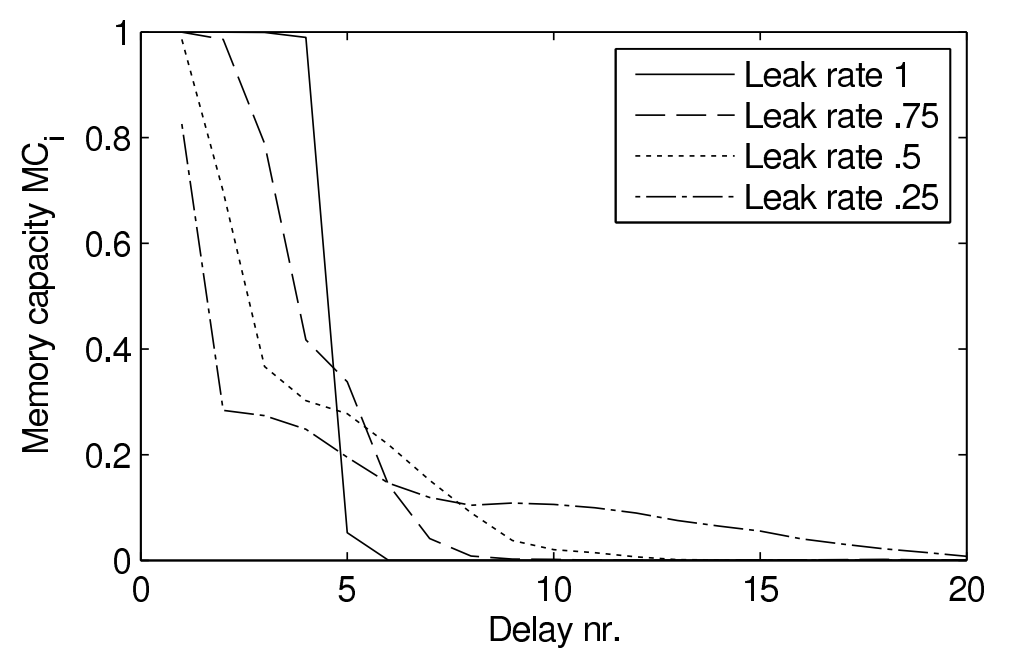
\includegraphics[width=0.55\textwidth]{img/leak_rate_verstraeten.png}
	
	\caption[Memory capacity for \acrshort{esn}s with different leak rates (from \citet{verstraeten_towards_2009}).]{
    		Memory capacity for \acrshort{esn}s with different leak rates (see Subsection \ref{subsection:esn}). Networks with a smaller leak rate show better long-term memory at the cost of decreased accuracy in short-term memory. This figure originally appeared in \citet{verstraeten_towards_2009}.
        }
	\label{fig:leak_rate_verstraeten}
\end{figure}


% This is shown in Figure 3.2. In this plot, the memory curve for a reservoir of 20 tanh nodes
% is shown with dierent leak rates. The plot shows that decreasing leak
% rates cause the memory curve to become flatter and wider. This means
% that the reservoir has worse memory of recent inputs, but better memory of inputs further in the past. Thus, by decreasing the leak rate we
% increase the longer-term memory of the nodes at the expense of precision
% in recalling the more recent inputs.